%% Credits of this ams template are with respective people. @Devansh1106 neither own this template nor the credits. 
\documentclass[12pt,reqno]{amsart}

\usepackage{graphicx}

\usepackage{amssymb}
\usepackage{amsthm}
\usepackage{mathrsfs}
\theoremstyle{plain}

\newtheorem*{thm*}{Theorem}
%% this allows for theorems which are not automatically numbered

\newtheorem{thm}{Theorem}
\newtheorem{lem}{Lemma}
\theoremstyle{definition}
\newtheorem{defn}{Definition}
\newtheorem{eg}{Example}
\newtheorem{rem}{Remark}
\usepackage{lineno}

%% The above lines are for formatting.  In general, you will not want to change these.


\title{Machine learning}
\author{Devansh Tripathi}

\begin{document}

\begin{abstract}
    We shall make some short notes from machine learning textbook by Hui Jiang.
\end{abstract}
\maketitle
\paragraph{\bf Discriminative models:} They simply assume that the input samples and  their corresponding output label are generated by an unknown function. These models attempt to estimate that function. It can be linear/bilinear/quadratic functions/neural networks (as universal function approximators). 
\paragraph{\bf Generative models:} They assume both the input variable $x$ and output variable $y$ are random variables and they try to figure out their joint probability distribution from the data.
\section{Dimensionality Reduction}
\subsection{Linear Dimensionality Reduction}
PCA aims to search for some orthogonal projection directions in the space that can achieve the {\bf maximum variance}. These directions are often called the {\bf principal components} of the original data distribution.

\par These principal components are used as basis vectors to constuct the linear subspace for dimensionality reduction.
\begin{figure}[!ht]
    \centerline{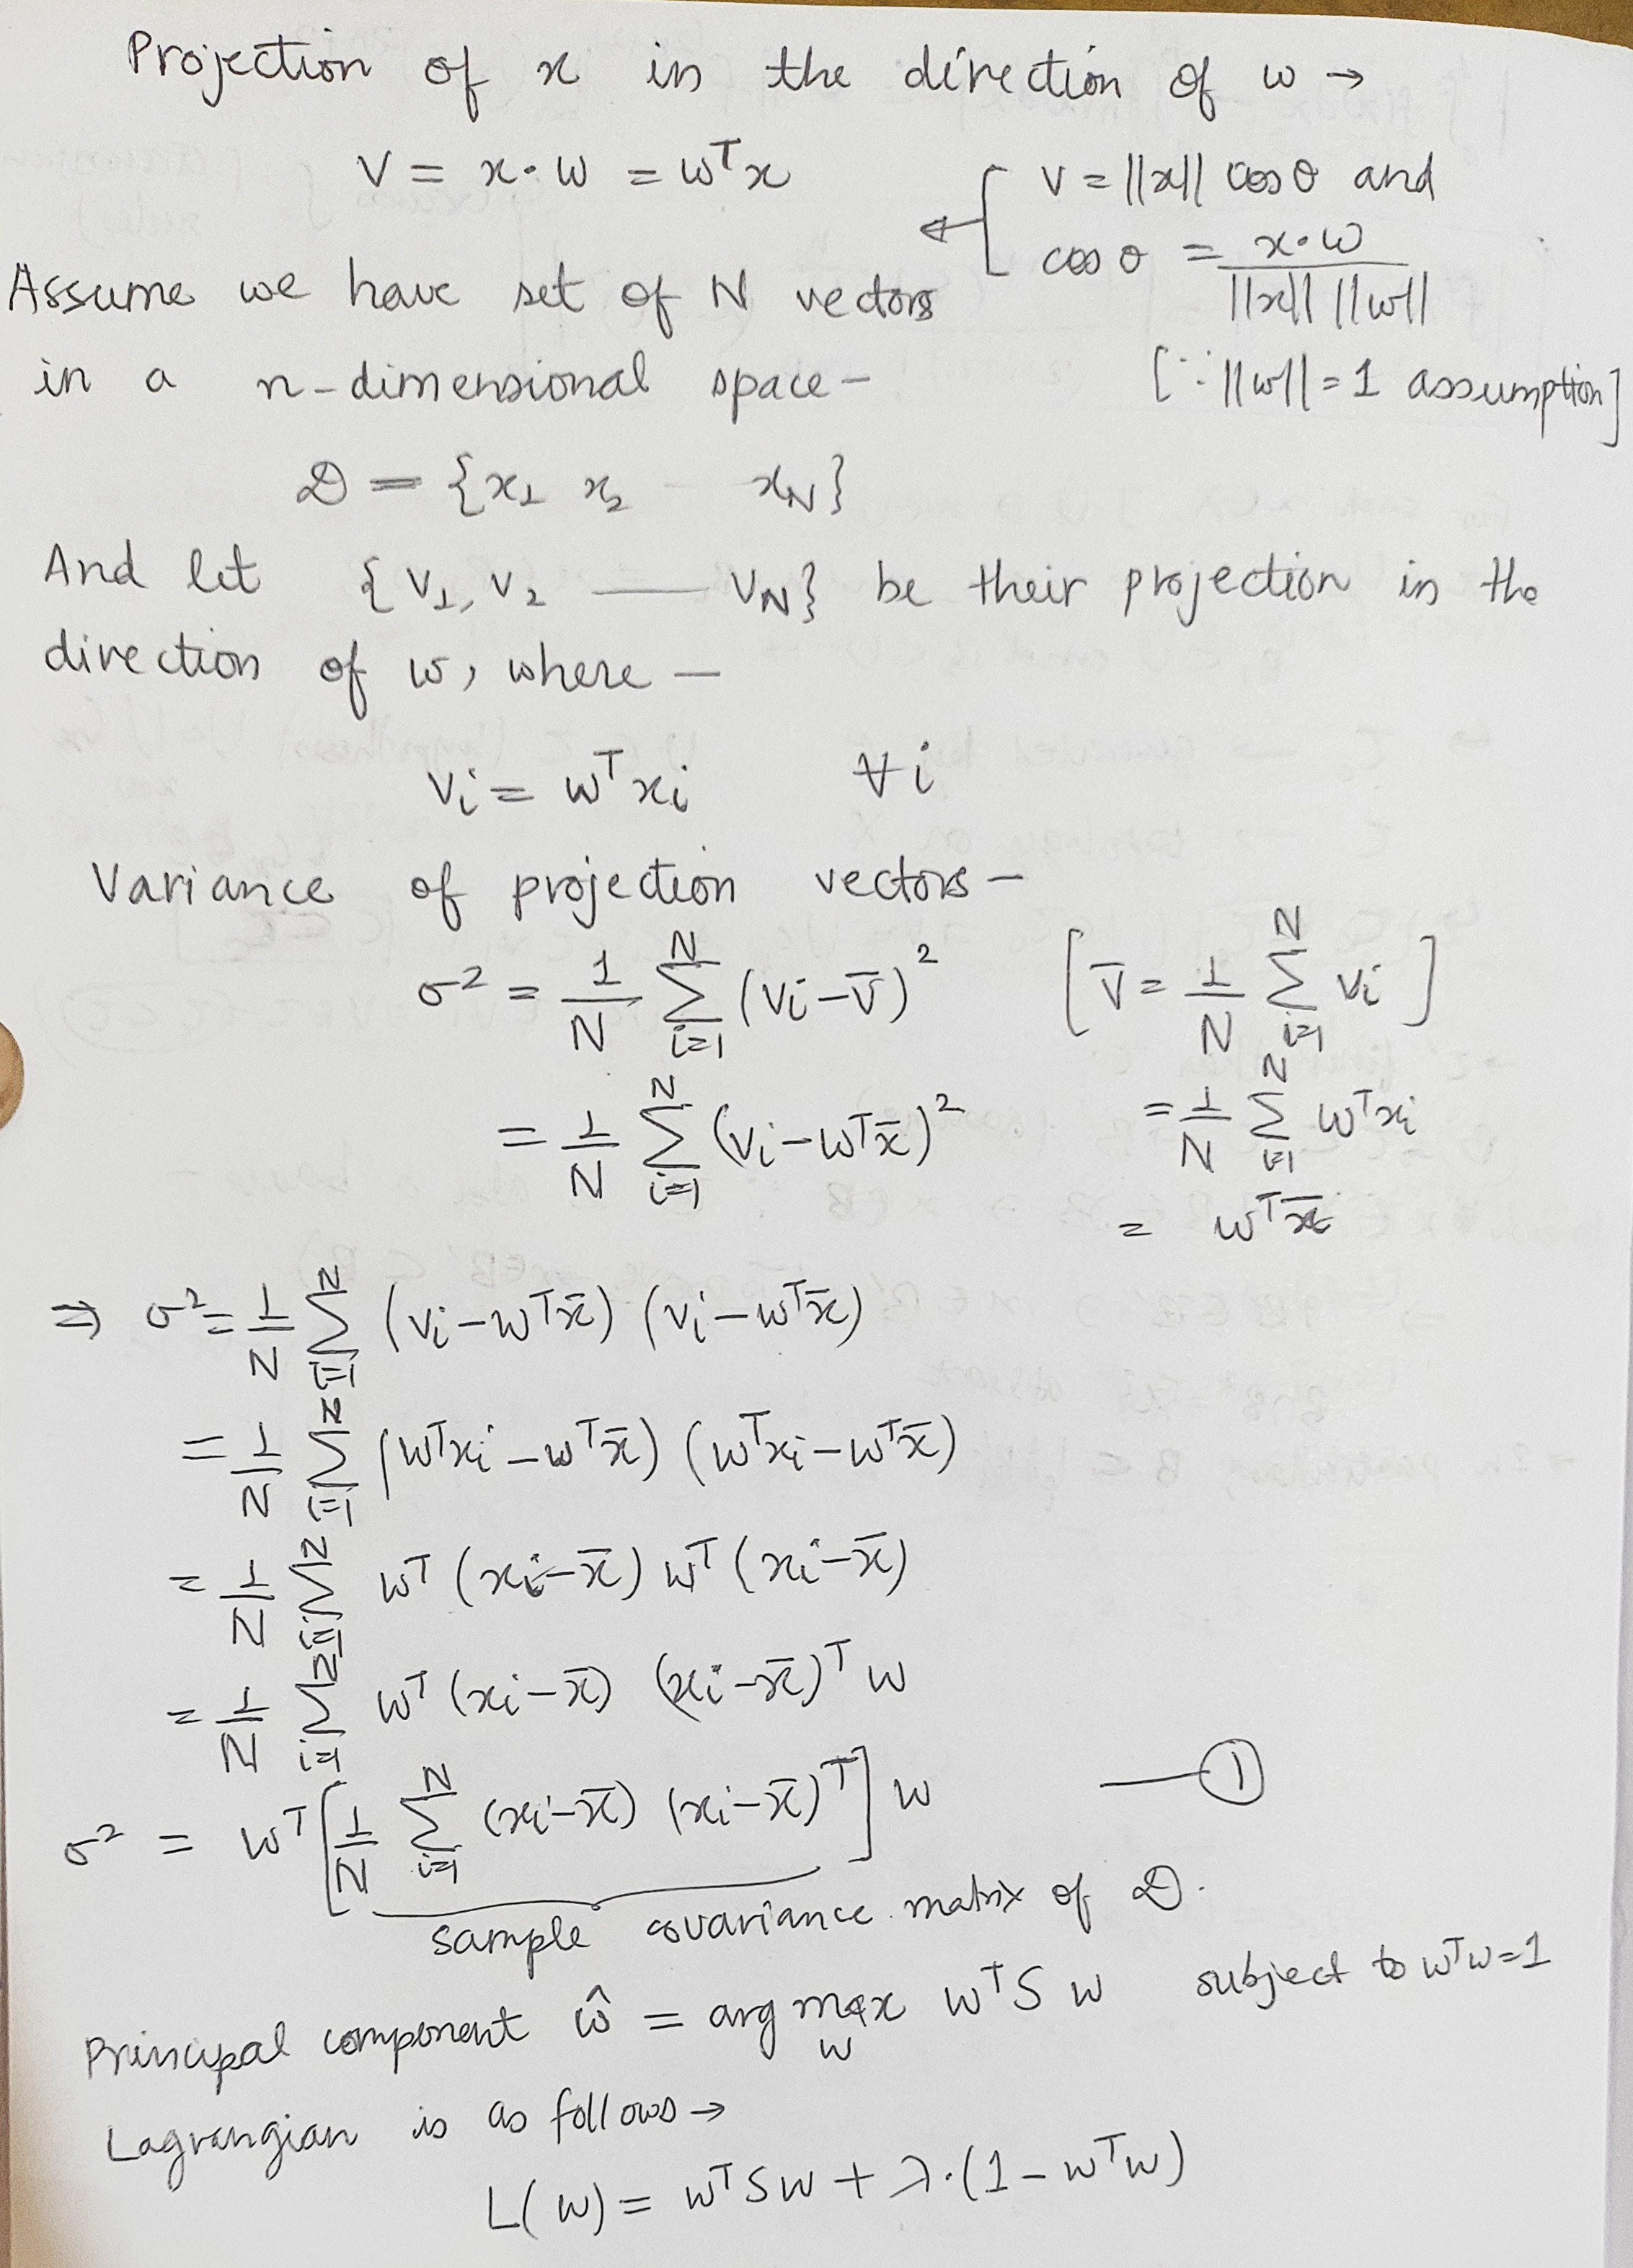
\includegraphics[scale=.17]{assests/1000124291.jpg}}
    \caption{Maximizing the variance}
    \label{fig1}
\end{figure}
\begin{figure}[!ht]
    \centerline{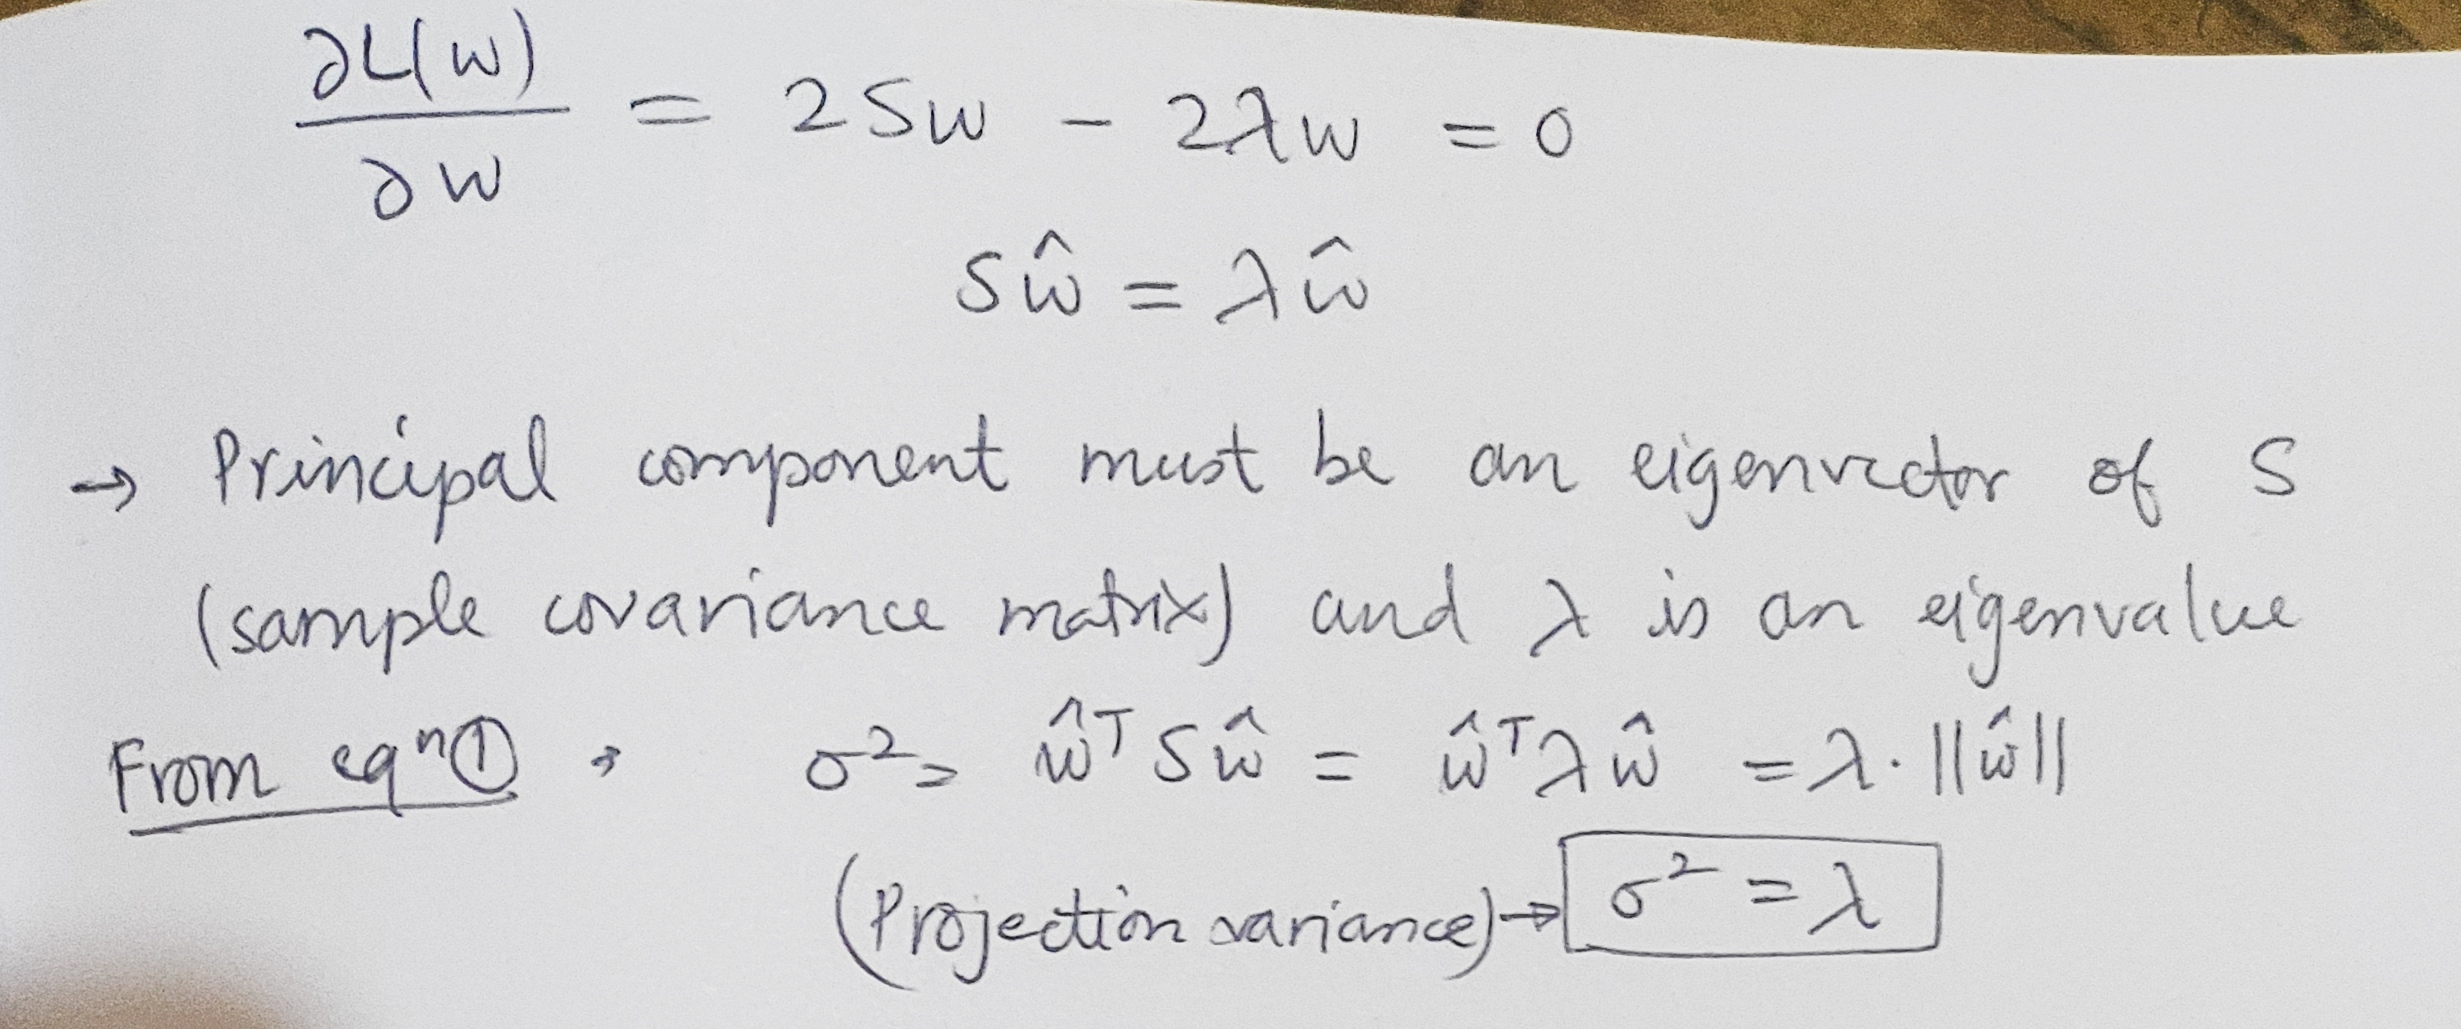
\includegraphics[scale=.17]{assests/1000124289.jpg}}
    \caption{Maximizing the variance}
    \label{fig2}
\end{figure}
\\ \par The result in figure \ref{fig2} shows that if we want to maximize the variance, we need to take the eigenvector corresponding to the {\bf maximum eigenvalue}. \par This result can be extended to the case where we want to map $x \in \mathbb{R}^n$ into a lower dimensional space $\mathbb{R}^m (m \ll n)$. {\it We need to take $m$ eigenvectors corresponding to top $m$ eigenvalues of the covariance matrix.} These $m$ eigenvectors are denoted as $\{\hat{w}_1, \hat{w}_2 \dots, \hat{w}_m\}$ then the matrix $A$ for transformation can be written as:
$$ A = \begin{bmatrix}
    - & \hat{w}^T_1 &- \\
    - & \hat{w}^T_2 & - \\
    \vdots \\
    - & \hat{w}^T_m & - 
\end{bmatrix}_{m \times n}
$$
Each eigenvector forms a row of $A$. Since, {\bf the covariance matrix of $S$ in figure \ref{fig1} is always symmetric and has full rank.} Therefore, we can compute $n$ different mutually orthogonal eigenvector for $S$. 
\paragraph{\bf Covariance Matrix} It is a generalization of the variance in the higher dimensions. Let ${\bf X = \{X_1, X_2, \dots, X_n\}}$ be a random variable then
$$ var(X) = cov(X,X) = E[(X-E[X])(X-E[X])^T] $$
The diagonal entries corresponds to variance ($cov[X_i,X_i] = var(X_i)$) and other than diagonal entries are covariances.
\begin{figure}[!ht]
    \centerline{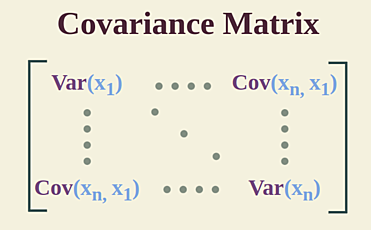
\includegraphics[scale=.5]{assests/covariance_matrix.png}}
    \caption{Covariance Matrix}
    \label{fig5}
\end{figure}
\paragraph{\bf Reconstruction of $x$ from $y$} Let $y = Ax$ where $A$ is the matrix of the transformation and $y$ is the transformed data. When we transform $n$ dimension data to $m$ dimensional space and $m \ll n$ then recovering $n$ dimension vector is not possible. If $m \approx n$ only then recovering is possible to some extent.
\begin{figure}[!ht]
    \centerline{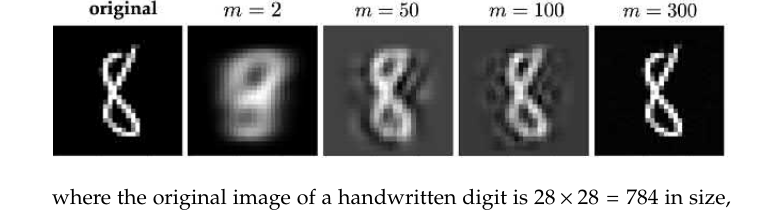
\includegraphics[scale=.5]{assests/recover.png}}
    \caption{Recovered images from lower dimensional space}
    \label{fig4}
\end{figure}
\begin{figure}[!ht]
    \centerline{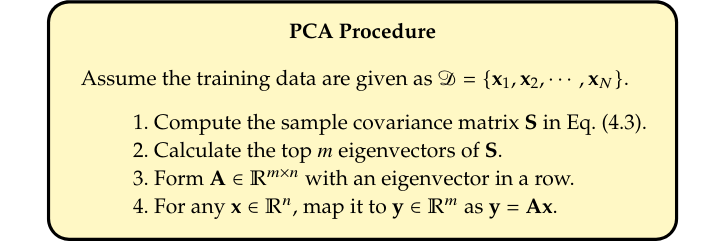
\includegraphics[scale=.6]{assests/summary_pca.png}}
    \caption{Summary of PCA}
    \label{fig3}
\end{figure}
This 
\end{document}